%%
%% This is file `mcmthesis-demo.tex',
%% generated with the docstrip utility.
%%
%% The original source files were:
%%
%% mcmthesis.dtx  (with options: `demo')
%% 
%% -----------------------------------
%% 
%% This is a generated file.
%% 
%% Copyright (C)
%%     2010 -- 2015 by Zhaoli Wang
%%     2014 -- 2015 by Liam Huang
%% 
%% This work may be distributed and/or modified under the
%% conditions of the LaTeX Project Public License, either version 1.3
%% of this license or (at your option) any later version.
%% The latest version of this license is in
%%   http://www.latex-project.org/lppl.txt
%% and version 1.3 or later is part of all distributions of LaTeX
%% version 2005/12/01 or later.
%% 
%% This work has the LPPL maintenance status `maintained'.
%% 
%% The Current Maintainer of this work is Liam Huang.

%% 
\documentclass{mcmthesis}
\mcmsetup{tcn = 233666, problem = B,
        sheet = true, titleinsheet = true, keywordsinsheet = true,
        titlepage = true, abstract = true}
\usepackage{palatino}
\usepackage{mwe}
\usepackage{amsmath}
\usepackage{indentfirst}
\usepackage{graphicx}
\setlength{\parindent} {2em}
\title{Sudoku Analyzing}
\author{Kai Feng, Song Lu, Yutao Zeng }
\date{\today}
\begin{document}
\begin{abstract}
here is the abstract!~!!
\begin{keywords}
keyword1; keyword2
\end{keywords}
\end{abstract}
\maketitle

\section{Introduction}
\subsection{Statement of Problem}
Our job is to develop an algorithm which would construct Sudoku puzzles of varying difficulty.In paricular, 
\subsection{Sudoku Introduction}
Sudoku, is a logic-based,combinatorial number-placement puzzle. The objextive is to fill a $9\times9$ grid with digits so that each column, each row, and each of the nine $3\times3$ subgrids that compose the grid contains all of the digits from 1 to 9. The puzzle setter provides a partially completed grid, which for a well-posed puzzle has a unique solution. Fig.1 is a typical example of sudoku puzzle.\newline \par 

\centerline{
	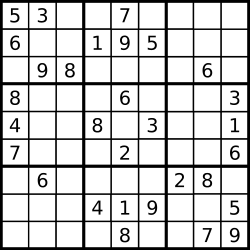
\includegraphics[width = 6cm]{figures/sudoku.png}
}
\centerline{Fig.1 Typical sudoku puzzle}

\indent Completed games are always a type of Latin square with an additional constraint on the contents of individual regions. For example, the same single integer may not appear twice in the same row, column, or any of the nine $3\times3$ subregions of the $9\times9$ playing board.\newline

\centerline{
	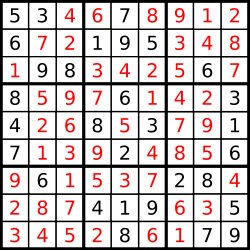
\includegraphics[width = 6cm]{figures/sudoku_complete.png}
}
\centerline{Fig.2 The same puzzle with solution numbers marked in red}

\subsection{Notations and Terminologies}
It is difficult to discuss our solution to the proposed problem without understanding some common
terminology. Moreover, since we will apply more mathematical formalism here than in most documents dealing with sudoku, it will be helpful to introduce notational conventions.
% \begin{table}[!hbp]
% \begin{tabular}{|c|c|c|c|c|}
% \hline
% 1-1 & 1-2 & 1-3 & 1-4 & 1-5 \\
% 2-1 & 2-2 & 2-3 & 2-4 & 2-5 \\
% \end{tabular}
% \caption{example of table}
% \end{table}

\begin{itemize}
	\item \textbf{Cell.} The basic unit of Sudoku puzzle. A square in the grid which may contain one digit(1-9). The grid is composed of 81 cells.

	\item \textbf{Block.} A $3\times3$ array of cells. Normally, the boundaries of the blocks are marked by slightly darker or thicker lines than the lines separating the cells. The grid is composed of 9 non-overlapping blocks. Each block must contain all the digits(form 1 to 9) and may not contain more than one of each digit.

	\item \textbf{Column.} A verticle line of 9 cells. The grid is composed of 9 columns. Each column must contain all the digits(1-9) and may not contain more than one of each digit.

	\item \textbf{Row.} A horizontal line of 9 cells. The grid is composed of 9 rows. Each row must contain all the digits (1-9) and may not contain more than one of each digit.

	\item \textbf{Grid.} The $9\times9$ array of cells that compose a Sudoku puzzle. The grid contains 9 rows, 9 columns and 9 blocks.

	\item \textbf{Puzzle.} A $9\times9$ matrix of cells, with at least one empty and at least one filled cell. For our purposes, we impose the additional requirement that all puzzles have exactly one solution. 	
\end{itemize}


\section{Analysis of the Problem}
\begin{figure}[h]
\small
\centering
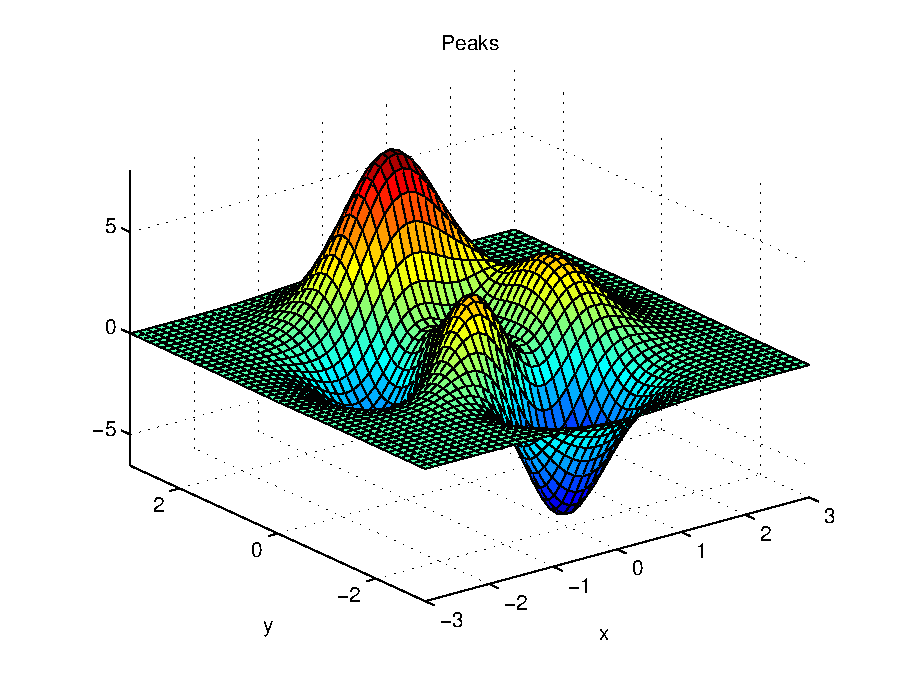
\includegraphics[width=12cm]{mcmthesis-aaa.eps}
\caption{aa} \label{fig:aa}
\end{figure}

\lipsum[8] \eqref{aa}
\begin{equation}
a^2 \label{aa}
\end{equation}

\[
  \begin{pmatrix}{*{20}c}
  {a_{11} } & {a_{12} } & {a_{13} }  \\
  {a_{21} } & {a_{22} } & {a_{23} }  \\
  {a_{31} } & {a_{32} } & {a_{33} }  \\
  \end{pmatrix}
  = \frac{{Opposite}}{{Hypotenuse}}\cos ^{ - 1} \theta \arcsin \theta
\]
\lipsum[9]

\[
  p_{j}=\begin{cases} 0,&\text{if $j$ is odd}\\
  r!\,(-1)^{j/2},&\text{if $j$ is even}
  \end{cases}
\]

\lipsum[10]

\[
  \arcsin \theta  =
  \mathop{{\int\!\!\!\!\!\int\!\!\!\!\!\int}\mkern-31.2mu
  \bigodot}\limits_\varphi
  {\mathop {\lim }\limits_{x \to \infty } \frac{{n!}}{{r!\left( {n - r}
  \right)!}}} \eqno (1)
\]

\section{Matrix Design}

\section{The Model Results}

\section{Validating the Model}
talk with data

\section{Conclusions}
in short but accurate

\section{A Summary}
\lipsum[6]

\section{Evaluate of the Mode}
\subsection{Advantage of the Model}
\subsection{Disadvantage of the Model}

\section{Strengths and weaknesses}
\lipsum[12]

\subsection{Strengths}
\begin{itemize}
\item \textbf{Applies widely}\\
This  system can be used for many types of airplanes, and it also
solves the interference during  the procedure of the boarding
airplane,as described above we can get to the  optimization
boarding time.We also know that all the service is automate.
\item \textbf{Improve the quality of the airport service}\\
Balancing the cost of the cost and the benefit, it will bring in
more convenient  for airport and passengers.It also saves many
human resources for the airline. \item \textbf{}
\end{itemize}

\begin{thebibliography}{99}
\bibitem{1} D.~E. KNUTH   The \TeX{}book  the American
Mathematical Society and Addison-Wesley
Publishing Company , 1984-1986.
\bibitem{2}Lamport, Leslie,  \LaTeX{}: `` A Document Preparation System '',
Addison-Wesley Publishing Company, 1986.
\bibitem{3}\url{http://www.latexstudio.net/}
\bibitem{4}\url{http://www.chinatex.org/}
\end{thebibliography}

\begin{appendices}

\section{First appendix}

\lipsum[13]

Here are simulation programmes we used in our model as follow.\\

\textbf{\textcolor[rgb]{0.98,0.00,0.00}{Input matlab source:}}
\lstinputlisting[language=Matlab]{./code/mcmthesis-matlab1.m}

\section{Second appendix}

some more text \textcolor[rgb]{0.98,0.00,0.00}{\textbf{Input C++ source:}}
\lstinputlisting[language=C++]{./code/mcmthesis-sudoku.cpp}

\end{appendices}
\end{document}

%% 
%% This work consists of these files mcmthesis.dtx,
%%                                   figures/ and
%%                                   code/,
%% and the derived files             mcmthesis.cls,
%%                                   mcmthesis-demo.tex,
%%                                   README,
%%                                   LICENSE,
%%                                   mcmthesis.pdf and
%%                                   mcmthesis-demo.pdf.
%%
%% End of file `mcmthesis-demo.tex'.
